
Expression templates are a metaprogramming technique that enables lazy evaluation of a computation at compile-time. This helps to avoid inefficient operations that occur at runtime. However, this does not come for free, as expression templates require more code and can be cumbersome to read or understand. They are often used in the implementation of linear algebra libraries.

Before seeing how expression templates are implemented, let’s understand what is the problem they solve. For this, let’s suppose we want to do some operations with matrices, for which we implemented the basic operations, addition, subtraction, and multiplication (either of two matrices or of a scalar and a matrix). We can have the following expressions:

\begin{lstlisting}[style=styleCXX]
auto r1 = m1 + m2;
auto r2 = m1 + m2 + m3;
auto r3 = m1 * m2 + m3 * m4;
auto r4 = m1 + 5 * m2;
\end{lstlisting}

In this snippet, m1, m2, m3, and m4 are matrices; similarly, r1, r2, r3, and r4 are matrices that result from performing the operations on the right side. The first operation does not pose any problems: m1 and m2 are added and the result is assigned to r1. However, the second operation is different because there are three matrices that are added. That means m1 and m2 are added first and a temporary is created, which is then added to m3 and the result assigned to r2.

For the third operation, there are two temporaries: one for the result of multiplying m1 and m2 and one for the result of multiplying m3 and m4; these two are then added and the result is assigned to r3. Finally, the last operation is similar to the second, meaning that a temporary object results from the multiplication between the scalar 5 and the matrix m2, and then this temporary is added to m1 and the result assigned to r4.

The more complex the operation, the more temporaries are generated. This can affect performance when the objects are large. Expression templates help to avoid this by modeling the computation as a compile-time expression. The entire mathematical expression (such as m1 + 5 * m2) becomes a single expression template computed when the assignment is evaluated and without the need for any temporary object.

To demonstrate this, we will build some examples using vectors not matrices because these are simpler data structures, and the point of the exercise is not to focus on the representation of data but on the creation of expression templates. In the following listing, you can see a minimal implementation of a vector class that provides several operations:

\begin{itemize}
\item
Constructing an instance from an initializer list or from a value representing a size (no initializing values)

\item
Retrieving the number of elements in the vector

\item
Element access with the subscript operator ([])
\end{itemize}

The code goes as follows:

\begin{lstlisting}[style=styleCXX]
template<typename T>
struct vector
{
	vector(std::size_t const n) : data_(n) {}
	
	vector(std::initializer_list<T>&& l) : data_(l) {}
	
	std::size_t size() const noexcept
	{
		return data_.size();
	}

	T const & operator[](const std::size_t i) const
	{
		return data_[i];
	}

	T& operator[](const std::size_t i)
	{
		return data_[i];
	}

private:
	std::vector<T> data_;
};
\end{lstlisting}

This looks very similar to the std::vector standard container, and, in fact, it uses this container internally to hold the data. However, this aspect is irrelevant to the problem we want to solve. Remember we are using a vector and not a matrix because it’s easier to represent in a few lines of code. Having this class, we can define the necessary operations: addition and multiplication, both between two vectors and between a scalar and a vector:

\begin{lstlisting}[style=styleCXX]
template<typename T, typename U>
auto operator+ (vector<T> const & a, vector<U> const & b)
{
	using result_type = decltype(std::declval<T>() +
	std::declval<U>());
	vector<result_type> result(a.size());
	for (std::size_t i = 0; i < a.size(); ++i)
	{
		result[i] = a[i] + b[i];
	}
	return result;
}

template<typename T, typename U>
auto operator* (vector<T> const & a, vector<U> const & b)
{
	using result_type = decltype(std::declval<T>() +
	std::declval<U>());
	vector<result_type> result(a.size());
	for (std::size_t i = 0; i < a.size(); ++i)
	{
		result[i] = a[i] * b[i];
	}
	return result;
}

template<typename T, typename S>
auto operator* (S const& s, vector<T> const& v)
{
	using result_type = decltype(std::declval<T>() +
	std::declval<S>());
	vector<result_type> result(v.size());
	for (std::size_t i = 0; i < v.size(); ++i)
	{
		result[i] = s * v[i];
	}
	return result;
}
\end{lstlisting}

These implementations are relatively straightforward and should not pose a problem to understand at this point. Both the + and * operators take two vectors of potentially different types, such as vector<int> and vector<double>, and return a vector holding elements of a result type. This is determined by the result of adding two values of the template types T and U, using std::declval. This has been discussed in Chapter 4, Advanced Template Concepts. A similar implementation is available for multiplying a scalar and a vector. Having these operators available, we can write the following code:

\begin{lstlisting}[style=styleCXX]
vector<int> v1{ 1,2,3 };
vector<int> v2{ 4,5,6 };
double a{ 1.5 };

vector<double> v3 = v1 + a * v2; // {7.0, 9.5, 12.0}
vector<int> v4 = v1 * v2 + v1 + v2; // {9, 17, 27}
\end{lstlisting}

As previously explained, this will create one temporary object while computing v3 and two temporaries while computing v4. These are exemplified in the following diagrams. The first shows the first computation, v3 = v1 + a * v2:

\begin{center}
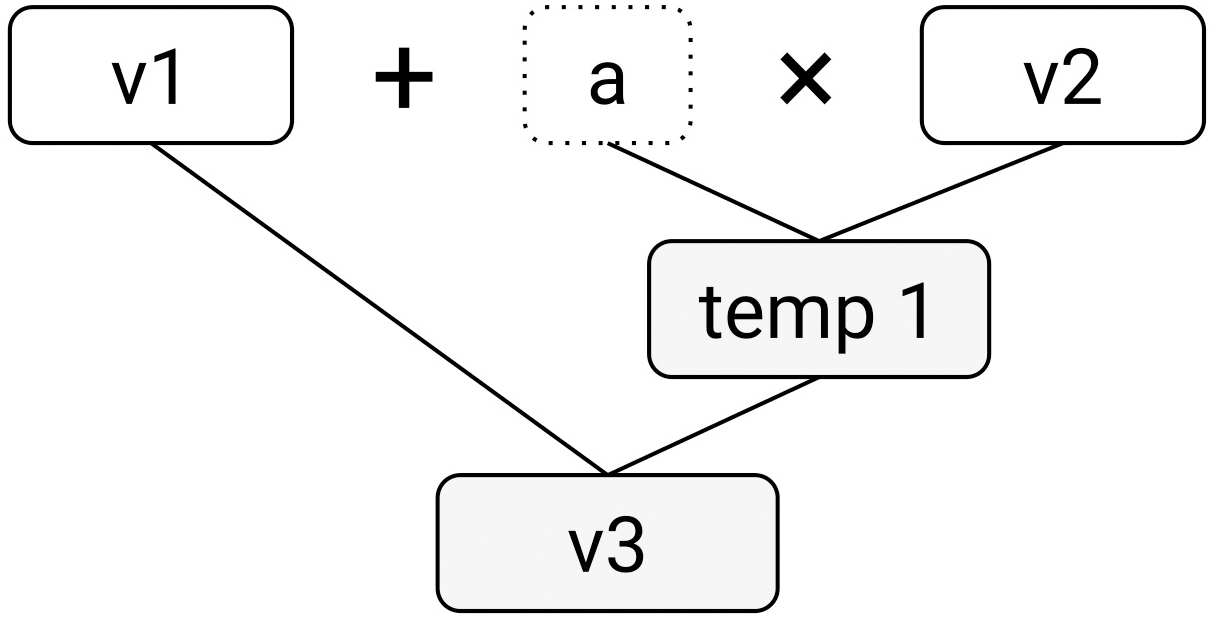
\includegraphics[width=0.5\textwidth]{content/3/chapter7/images/2.png}\\
Figure 7.2: A conceptual representation of the first expression
\end{center}

The second diagram, shown next, presents a conceptual representation of the computation of the second expression, v4 = v1 * v2 + v1 + v2:

\begin{center}
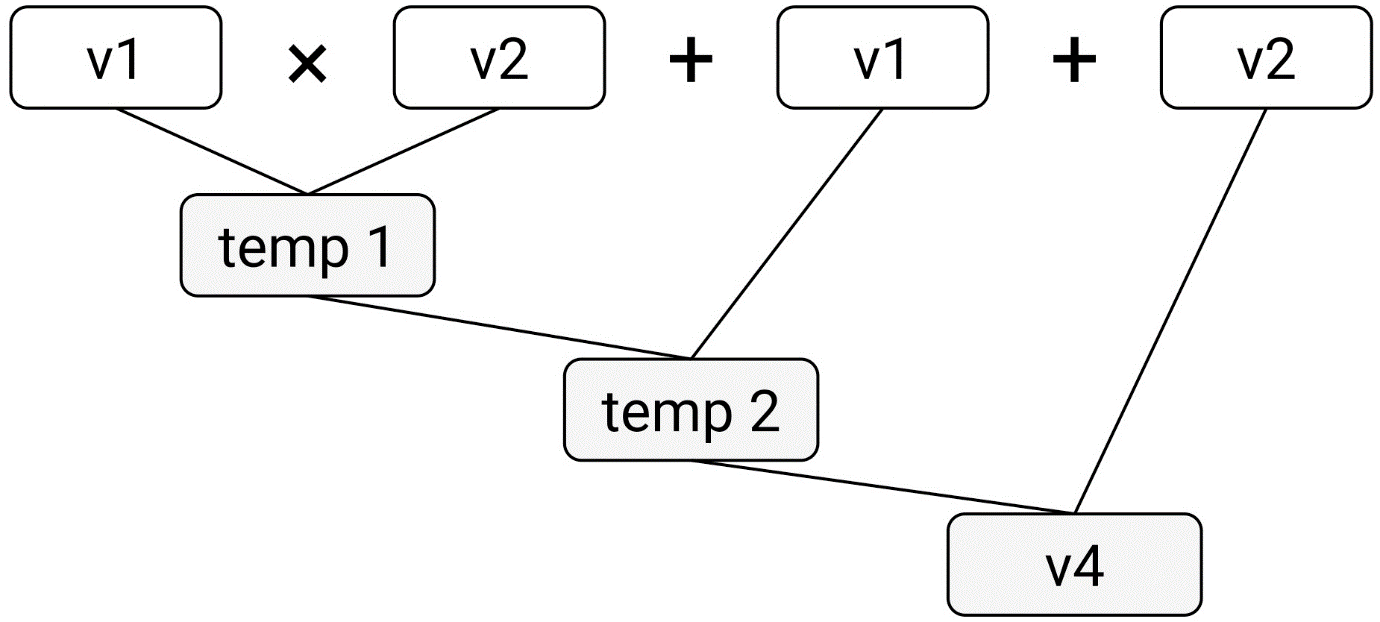
\includegraphics[width=0.5\textwidth]{content/3/chapter7/images/3.png}\\
Figure 7.3: A conceptual representation of the second expression
\end{center}

In order to avoid these temporaries, we can rewrite the implementation of the vector class using the expression templates pattern. This requires several changes:

\begin{itemize}
\item
Defining class templates to represent an expression between two objects (such as the expression of adding or multiplying two vectors).

\item
Modifying the vector class and parameterize the container for its internal data, which by default would be a std::vector as previously but can also be an expression template.

\item
Changing the implementation of the overloaded + and * operators.
\end{itemize}

Let’s see how this is done, starting with the vector implementation. Here is the code:

\begin{lstlisting}[style=styleCXX]
template<typename T, typename C = std::vector<T>>
struct vector
{
	vector() = default;
	
	vector(std::size_t const n) : data_(n) {}
	
	vector(std::initializer_list<T>&& l) : data_(l) {}
	
	
	vector(C const & other) : data_(other) {}
	template<typename U, typename X>
	vector(vector<U, X> const& other) : data_(other.size())
	{
		for (std::size_t i = 0; i < other.size(); ++i)
		data_[i] = static_cast<T>(other[i]);
	}

	template<typename U, typename X>
	vector& operator=(vector<U, X> const & other)
	{
		data_.resize(other.size());
		for (std::size_t i = 0; i < other.size(); ++i)
			data_[i] = static_cast<T>(other[i]);
		return *this;
	}

	std::size_t size() const noexcept
	{
		return data_.size();
	}
	
	T operator[](const std::size_t i) const
	{
		return data_[i];
	}

	T& operator[](const std::size_t i)
	{
		return data_[i];
	}

	C& data() noexcept { return data_; }
	
	C const & data() const noexcept { return data_; }
	
private:
	C data_;
};
\end{lstlisting}

In addition to the operations available in the initial implementation, this time we have also defined the following:

\begin{itemize}
\item
A default constructor

\item
A conversion constructor from a container

\item
A copy constructor from a vector containing elements of a potentially different type

\item
A copy-assignment operator from a vector containing elements of a potentially different type

\item
Member function data that provides access to the underlaying container holding the data
\end{itemize}

An expression template is a simple class template that stores two operands and provides a way to perform the evaluation of the operation. In our case, we need to implement expressions for adding two vectors, multiplying two vectors, and multiplying a scalar and a vector. Let’s look at the implementation of the expression template for adding two vectors:

\begin{lstlisting}[style=styleCXX]
template<typename L, typename R>
struct vector_add
{
	vector_add(L const & a, R const & b) : lhv(a), rhv(b) {}
	
	auto operator[](std::size_t const i) const
	{
		return lhv[i] + rhv[i];
	}

	std::size_t size() const noexcept
	{
		return lhv.size();
	}

private:
	L const & lhv;
	R const & rhv;
};
\end{lstlisting}

This class stores constant references to two vectors (or, in fact, any type that overloads the subscript operator and provides a size member function). The evaluation of the expression occurs in the overloaded subscript operator but not for the entire vector; only the elements at the indicated index are added.

Notice that this implementation does not handle vectors of different sizes (which you can take as an exercise to change). However, it should be easy to understand the lazy nature of this approach since the addition operation only occurs when invoking the subscript operator.

The multiplication expression templates for the two operations we need are implemented in a similar fashion. The code is shown in the next listing:

\begin{lstlisting}[style=styleCXX]
template<typename L, typename R>
struct vector_mul
{
	vector_mul(L const& a, R const& b) : lhv(a), rhv(b) {}
	
	auto operator[](std::size_t const i) const
	{
		return lhv[i] * rhv[i];
	}

	std::size_t size() const noexcept
	{
		return lhv.size();
	}

private:
	L const & lhv;
	R const & rhv;
};

template<typename S, typename R>
struct vector_scalar_mul
{
	vector_scalar_mul(S const& s, R const& b) :
		scalar(s), rhv(b)
	{}
	
	auto operator[](std::size_t const i) const
	{
		return scalar * rhv[i];
	}

	std::size_t size() const noexcept
	{
		return rhv.size();
	}

private:
	S const & scalar;
	R const & rhv;
};
\end{lstlisting}

The last part of the change is to modify the definition of the overloaded + and * operators, which is as follows:

\begin{lstlisting}[style=styleCXX]
template<typename T, typename L, typename U, typename R>
auto operator+(vector<T, L> const & a,
vector<U, R> const & b)
{
	using result_type = decltype(std::declval<T>() +
								 std::declval<U>());
	return vector<result_type, vector_add<L, R>>(
		vector_add<L, R>(a.data(), b.data()));
}

template<typename T, typename L, typename U, typename R>
auto operator*(vector<T, L> const & a,
vector<U, R> const & b)
{
	using result_type = decltype(std::declval<T>() +
								 std::declval<U>());
	return vector<result_type, vector_mul<L, R>>(
		vector_mul<L, R>(a.data(), b.data()));
}

template<typename T, typename S, typename E>
auto operator*(S const& a, vector<T, E> const& v)
{
	using result_type = decltype(std::declval<T>() +
								 std::declval<S>());
	return vector<result_type, vector_scalar_mul<S, E>>(
		vector_scalar_mul<S, E>(a, v.data()));
}
\end{lstlisting}

Although the code is more complex when implementing this pattern, the client code does not need to change. The snippet showed earlier works without any modifications but in a lazy manner. The evaluation of each element in the result is triggered by the invocation of the subscript operator that occurs in the copy-constructor and copy-assignment operator of the vector class.

If this pattern looks cumbersome to you, there is the alternative of something better: the ranges library.

\subsubsubsection{7.6.1\hspace{0.2cm}Using ranges as an alternative to expression templates}

One of the major features of C++20 is the ranges library. A range is a generalization of a container - a class that allows you to iterate over its data (elements). A key element of the range library is the views. These are non-owning wrappers of other ranges that transform the underlying range through some operation.

Moreover, they are lazy-evaluated and the time to construct, copy, or destroy them does not depend on the size of the underlying range. The lazy evaluation (the fact that transformations are applied to elements at the moment they are requested, not when the view is created) is a key feature of the library. However, that is exactly what the expression templates are also providing. As a result, many uses of the expression templates can be replaced with ranges. Ranges will be discussed in detail in the next chapter.

The C++ ranges library is based on the range-v3 library created by Eric Niebler. This library is available at \url{https://github.com/ericniebler/range-v3/}. Using range-v3, we can write the following code to perform the operation v1 + a * v2:

\begin{lstlisting}[style=styleCXX]
namespace rv = ranges::views;
std::vector<int> v1{ 1, 2, 3 };
std::vector<int> v2{ 4, 5, 6 };
double a { 1.5 };

auto sv2 = v2 |
		   rv::transform([&a](int val) {return a * val; });
auto v3 = rv::zip_with(std::plus<>{}, v1, sv2);
\end{lstlisting}

There is no need for a custom implementation of a vector class; it just works with the std::vector container. There is no need to overload any operator also. The code should be easy to follow, at least if you have some familiarity with the ranges library. First, we create a view that transforms the elements of the v2 vector by multiplying each element with a scalar. Then, a second view is created that applies the plus operator on the elements of the v1 range and the view resulting from the previous operation.

Unfortunately, this code cannot be written in C++20 using the standard library, because the zip\_with view has not been included in C++20. However, this view will be available in C++23 under the name zip\_view. Therefore, in C++23, we will be able to write this code as follows:

\begin{lstlisting}[style=styleCXX]
namespace rv = std::ranges::views;
std::vector<int> v1{ 1, 2, 3 };
std::vector<int> v2{ 4, 5, 6 };
double a { 1.5 };

auto sv2 = v2 |
           rv::transform([&a](int val) {return a * val; });
auto v3 = rv::zip_wiew(std::plus<>{}, v1, sv2);
\end{lstlisting}

To conclude the discussion of the expression templates pattern, you should keep in mind the following takeaways: the pattern is designed to provide lazy evaluation for costly operations, and it does so at the expense of having to write more code (that is also arguably more cumbersome) and increased compile-times (since heavy template code will have an impact on that). However, as of C++20, a good alternative to this pattern is represented by the ranges library. We will learn about this new library in Chapter 9, The Ranges Library.

For the next and last section of this chapter, we will look at type lists.













